\section{Discussion}
\label{sec:discussion}

TODO

%We have presented CHAODA, a collection of five algorithms that exploit properties of a hierarchical cluster tree which represents an approximate manifold in $n$-dimensional space.
%The five algorithms are simple to implement on top of the manifold-learning framework we call CLAM\@.
%CHAODA builds on this framework for anomaly detection in much the same way as CHESS~\cite{ishaq2019entropy} did for accelerating approximate search.
%With CHESS, the geometric and topological properties of low fractal dimension and low metric entropy are advantages;
%indeed, CHESS does not offer asymptotic improvements over linear search if these properties are absent.
%CHAODA, on the other hand, while competitive with other state-of-the-art anomaly-detection approaches on ``easy'' datasets (we define as \textit{easy} any dataset where a one-class SVM performs well), outperforms other current methods when the data exhibit precisely those properties that CHESS exploits for acceleration.
%In particular, CHAODA outperforms other approaches on high-dimensional datasets, with the exception of the ``annthyroid'' dataset where iForest and AOD perform better.
%
%Except for the annthyroid dataset, the algorithms presented here outperform or at least nearly match all other approaches.
%CHAODA outperforms a 1-class SVM on every dataset, and of the datasets where AUC values were available for other results (20 datasets), CHAODA matches or exceeds the AUC of other approaches on 12 of them.
%On 5 of the remaining 8, CHAODA is close to the best-performing approach, typically within 1 and 3 percentage points.
%
%Several reasons may contribute to CHAODA's difficulty with the annthyroid dataset in particular.
%First, this dataset was specifically created for use with ANNs.
%Upon further investigation, it appears that these data may be in too few dimensions for CLAM to partition it into a useful manifold.
%In UMAP~\cite{mcinnes2018umap} projections we created on annthyroid Figure~\ref{fig:conclusions:umap-embeddings}, it can be clearly seen that the anomalous data appear to live directly on the manifold, with only a small pocket appearing to be distinctly off.
%In contrast, the wbc dataset, where CHAODA significantly outperforms HiCS~\cite{keller2012hics}, appears to have most of the outliers along the periphery of the manifold.
%This aligns well with our expectations of CHAODA\@.
%Indeed, the manifold being both learnable and distinctly separate from the anomalous data are mandatory properties for any of our approaches to be effective.
%Fortunately, we can see that these properties are apparent in all other datasets studied.
%
%\begin{figure*}
%    \centering
%    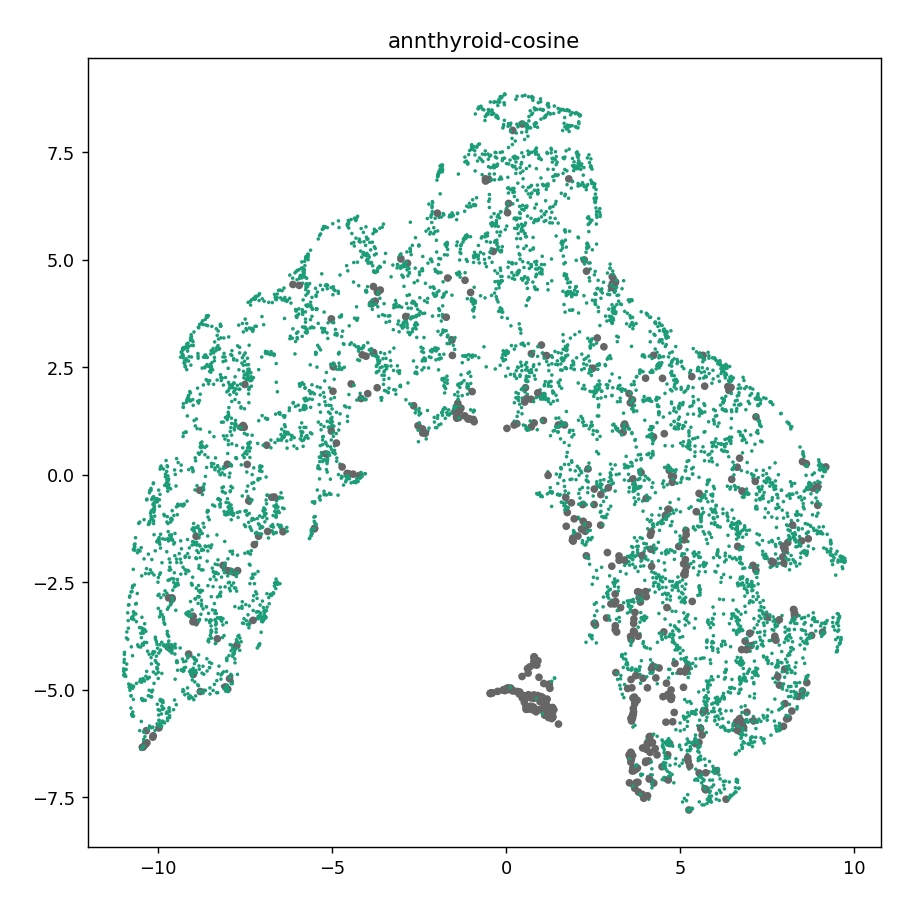
\includegraphics[width=2in]{images/umaps/annthyroid-cosine-umap2d.png}
%    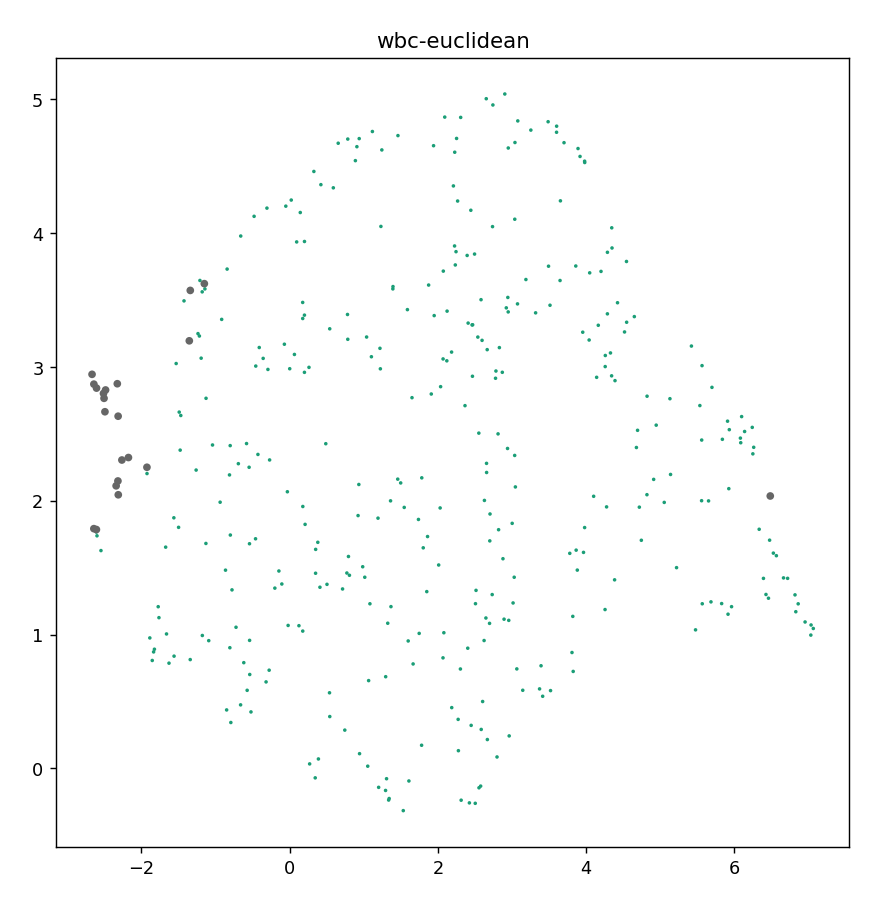
\includegraphics[width=2in]{images/umaps/wbc-euclidean-umap2d.png}
%    \caption{UMAP projection of Annthyroid (left) and WBC (right). Anomalies are in gray. Note that for Annthyroid, while there is a cluster of anomalies off the main manifold, many anomalies are distributed throughout the manifold. For WBC, the anomalies tend to be at the edge of the manifold.}
%    \label{fig:conclusions:umap-embeddings}
%\end{figure*}
%
%One current limitation in CHAODA is that the depth of the cluster tree at which anomaly detection performs best is not the same for every dataset;
%thus, our results could be seen as ``cherry-picking'' from a scattershot approach.
%The optimal depth varies because as depth increases, the induced graph ``shatters'', i.e.\ the number of components in the graph approaches the number of clusters in the graph.
%Future work should explore optimal stopping criteria so that we can automate stopping just before the graph shatters.
%Fortunately, as shown in Figures, for most datasets, performance is not overly sensitive to the choice of depth, especially for the Parent-Child algorithm.
%For now we can treat depth as a hyperparameter to all of the methods described, but a detailed analysis of possible stopping criteria for clustering depth will likely reveal automatic methods to find the optimal depth.
%
%% TODO: Need to look at local fractal dimension, or volume ratios, vs. optimal depth. Ideally we can say something like:
%% The strong correlation between local fractal dimension and optimal tree depth suggests a guideline for determining an optimal tree depth directly from the data.
%
%The choice of distance function also has a significant impact on anomaly-detection performance.
%In this case, domain knowledge is likely the best way to determine the distance function of choice.
%Future work will seek to explore a more diverse collection of domain-appropriate distance functions, such as Wasserstein distance on images, Levenshtein edit distance on strings, and Jaccard Index on the Maximal Common Sub-Graph of molecular structures.
%
%% TODO: Have we proved this?
%% Say something about applying CHAODA for inputs to an ANN, in particular detecting just-off-manifold malicious inputs, like the school bus / ostrich example.
%
%In conclusion, we have demonstrated that by learning approximate manifolds, we can exploit the embedded knowledge to implement simple algorithms capable of outperforming other state-of-the-art approaches to anomaly detection.
